\documentclass[10pt, landscape]{article}
\usepackage[scaled=0.92]{helvet}
\usepackage{calc}
\usepackage{multicol}
\usepackage{ifthen}
\usepackage[a4paper,margin=5mm,landscape]{geometry}
\usepackage{amsmath,amsthm,amsfonts,amssymb}
\usepackage{color,graphicx,overpic}
\usepackage{hyperref}
\usepackage{newtxtext} 
\usepackage{enumitem}
\usepackage{amssymb}
\usepackage[table]{xcolor}
\usepackage{vwcol}
\usepackage{tikz}
\usetikzlibrary{arrows.meta}
\usetikzlibrary{calc}
\usepackage{mathtools}
\usepackage{nicematrix}
\usepackage[T1]{fontenc} %%% <--- NOTE THIS
% for relations
\usepackage{cancel}
\usepackage{ mathrsfs }
\usepackage{listings}
\usepackage{background}
\setlist{nosep}

\usepackage{etoolbox}
\makeatletter
\preto{\@verbatim}{\topsep=0pt \partopsep=0pt }
\makeatother

\backgroundsetup{
scale=1,
color=black,
opacity=0.4,
angle=0,
contents={
  % 
\includegraphics[width=\paperwidth,height=\paperheight]{eldon.png}
  }
}

\pdfinfo{
  /Title (CS3211.pdf)
  /Creator (TeX)
  /Producer (pdfTeX 1.40.0)
  /Author (Seamus)
  /Subject (Example)
  /Keywords (pdflatex, latex,pdftex,tex)}

\lstset{language=Java,keywordstyle={\bfseries \color{black}}}

% Turn off header and footer
\pagestyle{empty}

\newenvironment{tightcenter}{%
  \setlength\topsep{0pt}
  \setlength\parskip{0pt}
  \begin{center}
}{%
  \end{center}
}

% redefine section commands to use less space
\makeatletter
\renewcommand{\section}{\@startsection{section}{1}{0mm}%
                                {-1ex plus -.5ex minus -.2ex}%
                                {0.5ex plus .2ex}%x
                                {\normalfont\large\bfseries}}
\renewcommand{\section}{\@startsection{section}{2}{0mm}%
                                {-1explus -.5ex minus -.2ex}%
                                {0.5ex plus .2ex}%
                                {\normalfont\normalsize\bfseries}}
\renewcommand{\subsection}{\@startsection{subsection}{3}{0mm}%
                                {-1ex plus -.5ex minus -.2ex}%
                                {1ex plus .2ex}%
                                {\normalfont\small\bfseries}}%
\renewcommand{\familydefault}{\sfdefault}
\renewcommand\rmdefault{\sfdefault}
% makes nested numbering (e.g. 1.1.1, 1.1.2, etc)
\renewcommand{\labelenumii}{\theenumii}
\renewcommand{\theenumii}{\theenumi.\arabic{enumii}.}
\renewcommand\labelitemii{•}
%  for logical not operator
\renewcommand{\lnot}{\mathord{\sim}}
\renewcommand{\bf}[1]{\textbf{#1}}
\newcommand{\abs}[1]{\vert #1 \vert}
\newcommand{\Mod}[1]{\ \mathrm{mod}\ #1}

\makeatother
\definecolor{myblue}{cmyk}{1,.72,0,.38}
\everymath\expandafter{\the\everymath \color{myblue}}
% Define BibTeX command
\def\BibTeX{{\rm B\kern-.05em{\sc i\kern-.025em b}\kern-.08em
    T\kern-.1667em\lower.7ex\hbox{E}\kern-.125emX}}
\let\iff\leftrightarrow
\let\Iff\Leftrightarrow
\let\then\rightarrow
\let\Then\Rightarrow

% Don't print section numbers
\setcounter{secnumdepth}{0}

\setlength{\parindent}{0pt}
\setlength{\parskip}{0pt plus 0.5ex}
%% this changes all items (enumerate and itemize)
\setlength{\leftmargini}{0.5cm}
\setlength{\leftmarginii}{0.5cm}
\setlist[itemize,1]{leftmargin=2mm,labelindent=1mm,labelsep=1mm}
\setlist[itemize,2]{leftmargin=4mm,labelindent=1mm,labelsep=1mm}

%My Environments
\newtheorem{example}[section]{Example}
% -----------------------------------------------------------------------

\begin{document}
\raggedright
\footnotesize
\begin{multicols*}{3}

% multicol parameters
% These lengths are set only within the two main columns
\setlength{\columnseprule}{0.25pt}
\setlength{\premulticols}{1pt}
\setlength{\postmulticols}{1pt}
\setlength{\multicolsep}{1pt}
\setlength{\columnsep}{2pt}

\begin{center}
    \fbox{%
        \parbox{0.8\linewidth}{\centering \textcolor{black}{
            {\Large\textbf{CS3211}}
            \\ \normalsize{AY25/26 Sem 2}}
            \\ {\footnotesize \textcolor{myblue}{by ngmh}} 
        }%
    }
\end{center}

\section{Introduction to Concurrency}

\begin{itemize}
    \item \textbf{Concurrency}: Multiple execution flows make progress at the same time by interleaving their executions or by executing instructions at exactly the same time
    \item \textbf{Parallelism}: Multiple tasks running simultaneously, at the exact same time
    \item Hardware threads dictate the amount of parallelism through parallel execution of multiple kernel threads
    \item Steps for Parallelisation
    \begin{itemize}
        \item Decomposition of computation
        \item Assigning tasks to threads
        \item Orchestration: Communication, synchronisation, scheduling
        \item Mapping of threads to physical cores
    \end{itemize}
    \item \textbf{Race Condition}: Timing or order of events affects outcome of executing concurrent code, not necessarily a flaw
    \item \textbf{Data Race}
    \begin{itemize}
        \item Multiple threads access a shared resource without any synchronisation AND at least one thread modifies it, causing UB
        \item Does not occur if both evaluations are on the same thread, both are atomic, or one of them happens before another
    \end{itemize}
    \item Use mutual exclusion to synchronise access to shared resources
    \item Other Mechanisms
    \begin{itemize}
        \item Locks: Primitive with minimal semantics, used as a building block
        \item Semaphores: Basic, easy to get the hang of but hard to program with
        \item Monitors: High level, requiring language support, implicit operations
        \item Messages: Simple model of communication based on atomic transfer of data across a channel
    \end{itemize}
    \item \textbf{Deadlock}: Execution where no progress is made when it should be possible
    \item Can either ignore it, prevent it, avoid it, or detect and recover from it
    \item \textbf{Starvation}: Thread is prevented from making progress because other threads have resource it requires and initial thread cannot acquire it, usually side effect of scheduling algorithm
\end{itemize}

\section{Threads and Synchronisation in Modern C++}
\begin{itemize}
    \item Code to Execution:
    \begin{itemize}
        \item Compilation and linking: Done by compiler
        \item Loading: Loader is usually specific to OS
        \item Execution: Coordinated by OS, program gets acccess to resources
    \end{itemize}
    \item C++ Building:
    \begin{itemize}
        \item Preprocessor replaces directives
        \item Compiler parses C++ code and converts it to assembly
        \item Assembler assembles code into machine code
        \item Linker produces final compilation output from object files
    \end{itemize}
    \item \textbf{Lifetimes}
    \begin{itemize}
        \item Begin when storage with proper alignment and size for its type is obtained, and initialisation is complete
        \item Ends when object is destroyed, or when destructor call starts, or the storage which the object occupies is released
        \item Lifetime of a reference begins when initialisation is complete and ends as if it were a scalar object
    \end{itemize}
    \item \textbf{Ownership}
    \begin{itemize}
        \item Owner is an object containing a pointer to an object allocated by new for which a delete is required
        \item Objects on the free store must have exactly one owner
        \item Thread instances own a resource, and instances of threads are movable but not copyable
    \end{itemize}
    \item \textbf{Structure of Program Data}
    \begin{itemize}
        \item Every variable is an object
        \item Every object occupies at least one memory location
        \item Fundamental types occupy exactly one memory location
        \item Adjacent bit fields are different memory locations but can be part of the same storage unit
    \end{itemize}
    \item \textbf{Invariants}: Statements always true about a particular data structure (might be broken during update)
    \item Wrap data structure with protection mechanism to prevent data races
    \item Mutexes provide mutual exclusion and serialisation where threads take turns to access the protected data
    \item Recommended usage: \verb|std::lock_guard| with RAII to unlock on destruction
    \item Don't pass pointers / references to protected data outside the scope of the lock
    \item Avoid nested locks and calling user-supplied code while holding a lock; acquire locks in a fixed order
    \item \textbf{Condition Variable}
    \begin{itemize}
        \item Associated with event or other condition; one or more threads can wait for condition to be satisfied
        \item When condition is satisfied, thread notifies one or more threads waiting on condition variable to wake up
        \item Condition check should not have side effects
        \item \textbf{Spurious Wake}: Waiting thread reacquires mutex and checks condition even though it is not notified
    \end{itemize}
\end{itemize}

\section{Atomics and Memory Model in C++}
\begin{itemize}
    \item Correctly synchronised program should behave as if memory operations are executed in an order that is equivalent to some sequentially consistent interleaved execution of memory operations of each thread, where each write appears to be atomic and globally visible to all processors
    \item Processor might reorder operations to improve efficiency
    \item Memory models provide a contract to programmers about what are the visible side effects of their memory operations
    \item \textbf{As-if Rule}
    \begin{itemize}
        \item The compiler is permitted to perform changes to the program as long as
        \item Accesses to volatile objects occur strictly according the semantics of the expressions in which they occur
        \item They are no reordered wrt other volatile access on the same thread
        \item At program termination, data written to files is exactly as if the program was simply executed
        \item Prompting text which is sent to interactive devices will be shown before the program waits for input
        \item Programs with UB are free from this rule
    \end{itemize}
\end{itemize}

\subsection{Atomics}
\begin{itemize}
    \item \verb|std::atomic| allows for low-level synchronisation, with operations that reduce to 1 or 2 CPU instructions
    \item Atomic operations are indivisible and always observed fully done/undone
    \item Atomic loads will retrieve either initial value of object or value stored by some modification
    \item A non-atomic operation might be seen as half-done by another thread
    \item Atomic types provide \verb|is_lock_free()| which checks if operations on a given type are done with atomic instructions, which might be emulated with internal mutexes
\end{itemize}

\subsection{Modification Order}
\begin{itemize}
    \item Consists of all writes to an object from all threads in the program, can vary
    \item With atomic variables, compiler ensures threads agree on MO for each variable, but might still have races
    \item Once a thread has seen an entry, subsequent reads and writes must return that entry or a later one in the MO
    \item Threads do not have to agree on separate objects
\end{itemize}

\subsection{Memory Order}
\begin{itemize}
    \item C++ Memory Order: Specifies how memory accesses are to be ordered around an atomic operation
\end{itemize}

\subsection{Sequentially Consistent Ordering}
\begin{itemize}
    \item Behaviour of program is consistent with a simple sequential view of the world
    \item All threads must agree on the same order of operations
    \item Operations within same thread can't be reordered
    \item Sequentially consistent store synchronises with sequentially consistent load of same variable that reads the value stored
    \item Performance penalty on weakly-ordered machine with many cores due to need for synchronisation
\end{itemize}

\subsection{Building Memory Model}
\begin{itemize}
    \item \textbf{Sequenced Before (sb)}:
    \begin{itemize}
        \item Within same thread, A is sequenced before B and will evaluate first
    \end{itemize}
    \item \textbf{Synchronises With (sw)}:
    \begin{itemize}
        \item Appears between atomic load and store operations (\texttt{acq + rel, seq\_cst})
        \item Suitably tagged write / store / release in thread A on a variable synchronises with suitably tagged read / load / acquire in another thread if acquire operations reads value of that write, depends on exact execution
        \item Can synchronise with seq\_cst as well
    \end{itemize}
    \item \textbf{Simply Happens Before (hb)}:
    \begin{itemize}
        \item A sb B
        \item A sw B
        \item A hb X, X hb B
    \end{itemize}
    \item \textbf{Strongly Happens Before}:
    \begin{itemize}
        \item Specifies which operations see the effects of other operations
        \item If A shb B, then A appears to be evaluated before B in all contexts
        \item A sb B
        \item A sw B, A, B are seq cst
        \item A sb X, X hb Y, Y sb B
        \item A shb X, X shb B
    \end{itemize}
    \item \textbf{Visible Side Effects}:
    \begin{itemize}
        \item A side effect of A on a write M is visible to a read B if
        \item A hb B and
        \item There is no other side effect X such that A hb X, X hb B
        \item The visible sequence of side effects is the longest contiguous subset of side effects to a scalar where B does not hb it
    \end{itemize}
    \item All modifications to an atomic variable occur in a total order which guarantees coherence
    \begin{itemize}
        \item WW: If evaluation A modifying atomic M hb B that modifies M, then A appears earlier than B in the MO for M
        \item RR: If computation A of atomic M hb a computation B on M, and if the value of A comes from write X on M, then the value of B is either X or the value stored by a side effect Y on M that appears after X in the MO for M
        \item RW: If computation A of atomic M hb operation B on M, then the value of A from a side effect X that appears earlier than B in the MO for M
        \item WR: If a side effect X on atomic M hb a computation B of M, then the evaluation B takes its value from X or from side effect Y that follows X in the MO for M
    \end{itemize}
    \item With non-seq cst orderings, there is no single global order of events, and threads only have to agree on MO of each variable
\end{itemize}

\subsection{Relaxed Ordering}
\begin{itemize}
    \item Operations with relaxed ordering do not participate in sw relationships
    \item Operations on same variable within a single thread still obey hb
    \item Accesses to a atomic variable from the same thread cannot be reordered
\end{itemize}

\subsection{Release-Acquire Ordering}
\begin{itemize}
    \item Use acquire and release memory ordering
    \item Atomic read-modify-write operations use either or both
    \item No total MO but introduces some synchronisation
    \item If a store in A with release and a load in B from the same variable with acquire and load in B reads a value written by a store in A, then the store in A sw the load in B
    \item All memory writes that hb the store in A are visible side effects in B; B must return value that A stored or a later value in the release sequence
    \item Other threads can still see different memory orders
    \item \textbf{Release Sequence}: The longest continuous subsequence of MO of M that consists of atomic RMW operations made to M after a release operation performed on it (can be relaxed!)
    \item Sequential Consistency for data race free programs is guaranteed if every atomic uses seq cst
\end{itemize}

\section{Concurrent Data Structures}
\begin{itemize}
    \item Goal: Multiple threads can access DS concurrently, and each thread sees a self-consistent view
    \item Thread-Safe DS should ensure no data is lost or corrupted, all invariants are upheld, and no problematic race conditions
    \item Mutexes are an easy way to provide serialisation but prevent true concurrent access
    \item Invariants are statements that are always true about a data structure, which might be broken during an update
    \item Constructors and destructors require exclusive access to DS; user has to ensure this and check whether DS can support assignment, swap, or copy construction
    \item Minimising the protected region results in fewer operations being serialised and greater potential for concurrency
    \item Locked-Based Concurrent DS: Ensure right mutex is locked when accessing and lock is held for minimum duration
    \item \textbf{Shared Pointer}: Holds a reference to pointed to data, keeps track of number of references (thread safe), automatically calling destructor once no longer referenced
    \item Fine-Grained Locking: Analyse constituent parts, associating one mutex with each distinct item, cannot continue using STL library
    \item To avoid deadlock, avoid nested locks, calling user supplied code while holding a lock, and always acquire locks in a fixed order
    \item Hand-Over-Hand Locking: Hold lock on current node, acquire next, release current, and continue; can cause deadlock on doubly-linked list
\end{itemize}

\subsection{Lock-Free Concurrent Data Structures}
\begin{itemize}
    \item Blocking Data Structures: Use mutexes, condition variables, futures for synchronisation
    \item Calls library functions which suspend execution until another thread performs an action
    \item Non-Blocking Data Structures: Do not use blocking library functions
    \item \textbf{Obstruction Free}: If all other threads are paused, any given thread will complete its operation in a bounded number of steps
    \item \textbf{Lock Free}: If multiple threads are operating on a data structure, then after a bounded number of steps, one of them will complete its operation (no deadlock)
    \item \textbf{Wait Free}: Every thread operating on a data structure will complete its operation in a bounded number of steps even if other threads are also operating (no starvation)
    \item Lock freedom allows individual threads to starve but guarantees system-wide throughput
    \item An algorithm is lock free if when the program threads are run for a sufficiently long time, at least one of them makes progress
    \item All wait-free algorithms are lock-free
    \item Notion of Progress: Function returns, or effects become visible
    \item More than one thread must be able to access the data structure concurrently
    \item Wait-Free data structures: Does not result in thread being subject to starvation due to loops, does not involve unbounded number of retries
    \item Might end up writing spin lock in essence
    \item Benefits: Maximum concurrency, more robust
    \item Cons: Might cause livelock, and decrease overall performance due to atomic operations
    \item Contention and Cache Ping Pong: Changes to data need time to propagate to cache on other core, which might cause a stop and wait depending on memory ordering
    \item False sharing can produce cache ping pong as well when accessing different memory locations on the same cache line within multiple threads
    \item Guidelines
    \begin{itemize}
        \item Prototype using sequentially consistent memory order
        \item Use lock-free memory reclamation scheme
        \item Watch out for ABA problem, prevalent with free lists (memory pools where nodes are recycled), solve using ABA counter
        \item Identify busy-wait loop and help the other thread
    \end{itemize}
    \item \textbf{ABA Problem}
    \begin{itemize}
        \item Compare and swap checks equality before swapping
        \item Suppose our data structure is modified before the CAS check, in a way such that the front happens to have the same address
        \item The check passes, although the next pointer on the swapped in node points to garbage
        \item To solve this, we can tag on generation counters so that even if the address is the same, the value is different
    \end{itemize}
    \item \textbf{Use After Free}
    \begin{itemize}
        \item If a thread gets preempted and the head gets deleted while it is trying to access, we might get a UAF
        \item Can choose to cause memory leak by not freeing anything
        \item Mark nodes for deletion while threads are trying to pop and free all at once
        \item Use reference counters and shared pointers
        \item Use hazard pointers to track threads and their references
        \item We choose to use a recycling center for nodes that should be "deleted", using a lock-free stack
        \item This recycling center also needs synchronisation with the queue
    \end{itemize}
    \item \textbf{Serialisation}
    \begin{itemize}
        \item Due to preempting, it is possible to create a scenario where the actual operations performed do not correspond to a serialised interleaving
        \item A pushes but gets interrupted, while B pushes in. B tries to pop, but since A is not finished, the queue still looks empty. Only after this try pop does A finish its work.
    \end{itemize}
\end{itemize}

\section{Testing and Debugging Multithreaded Programs}
\begin{itemize}
    \item Unwanted Blocking: Deadlock or livelock, or I/O and other external input
    \item Issues include data races, broken invariants, and lifetime issues
    \item Techniques for testing include stress testing, or special implementations for synchronisation primitives
    \item Test scalability and performance as well
    \item Useful tools for debugging memory issues include valgrind and sanitisers
    \item \textbf{Valgrind}
    \begin{itemize}
        \item Memcheck uses shadow memory which tracks information on memory usage and is used to detect and report incorrect accesses
        \item A-bit (Valid-Address): Corresponding byte accessible
        \item V-bit (Valid-Value): Corresponding bit initisalised
        \item Ensure each allocation is freed only once, each access is to a currently allocated space, and all reads are to locations already written
        \item Helgrind detects misuses of the pthread API, potential deadlock from lock ordering, and data races by intercepting function calls
        \item Builds directed graph of lock acquisition
        \item Checks order in which memory accesses happen, building DAG of happens before relationships which is used to flag cycles
    \end{itemize}
    \item \textbf{Sanitisers}
    \begin{itemize}
        \item Different types of sanitisers such as ASan (address), LSan (memory leak), TSan (thread), MSan (uninitialised memory), HWASAN, UBSan (undefined behaviour)
        \item ASan uses shadow values to represent individual bytes allocation
        \item Any aligned 8 bytes can have $N$ good bytes and $8-N$ bad bytes giving 9 states
        \item TSan adds checks at every function entry and exit
        \item It performs direct shadow mapping from actual addresses to shadow addresses
        \item Each 8 byte shadow cell represents one memory access, storing TID, Epoch, Position in word, IsWrite
        \item Uses this information to determines hb and races
    \end{itemize}
\end{itemize}

\section{Concurrency in Go}
\begin{itemize}
    \item Model programs in terms of tasks and synchronise them by making them communicate
    \item Many different concurrent designs possible
    \item Finer level of granularity enables program to scale dynamically when it runs due to amount of parallelism possible
    \item Task parallelism: Do the same work faster
    \item Data parallelism: Embarrassingly parallel algorithms, do more work in same amount of time
    \item Task dependency graph: DAG representing control dependencies between tasks
    \item Critical Path Length: Maximum / Slowest completion time
    \item Degree of Concurrency: Total Work / Critical Path Length
    \item Speedup: $S_p(n)=\frac{T_{best\_seq}(n)}{T_p(n)}$
    \item Amdahl's Law: $S_p(n)=\frac{1}{f+(1-f)/p} \leq \frac{1}{f}$, $f$ is sequential fraction
    \item Go is based on Communicating Sequential Processes
    \item Concurrency is found in Goroutines: independently running functions on OS threads
    \item Communication is found in Channels paired with select statements
    \item Goroutines follow the fork-join model and share the same address space
    \item Runtime multiplexes goroutines onto OS threads, decoupling concurrency from parallelism
    \item Goroutines are special coroutines (concurrent subroutines), preemptable
    \item Goroutines take a few kilobytes and are relatively lightweight but not garbage collected
    \item Channels are streams of information, are actually references to places in memory where the real channel resides
    \item Channels are typed, bi/unidirectional, and blocking
    \item Owner is the goroutine that instantiates, writes, and closes a channel
    \item Owners have write view into unidirection channels while utilisers only have read view
    \item Ownership increases safety
    The \texttt{select} statement allow sus to compose channels to form larger abstractions, similar to a \texttt{switch}
    \item \texttt{select} blocks if no channels are ready
    \item The Sync package provides typical synchronisation constructs which are used mostly in small scopes
    \item Go memory model specifies conditions under which reads of a variable can be guaranteed to observe values produced by writes to the same variable in different goroutines
    \item Go has DRF-SC
    \item Within a goroutine, reads and write follow sequenced before
    \item Read r is guaranteed to observe write w if w happens before r and any other write to the variable happens before w or after r
    \item \textbf{Happens before} is the transitive closure of the union of sequenced before and synchronised before
    \item \textbf{Synchronised before}:
    \begin{itemize}
        \item The \texttt{go} statement starting a new goroutine sb the goroutine's execution
        \item The exit of gorutine is not guaranteed to be sb any event
        \item Send on a channel is sb completion of corresponding receive
        \item Closing of channel is sb receive that returns zero value
        \item Receive from unbuffered channel is sb completion of corresponding send
        \item kth receive on a channel with capacity C is sb (k+C)th send from that channel completing
    \end{itemize}
\end{itemize}

\section{Concurrency Patterns in Go}
\begin{itemize}
    \item \textbf{Confinement}:
    \begin{itemize}
        \item Achieve safe operation via synchronisation
        \item Safe concurrency with good performance through immutable or protected data
        \item Ad-hoc confinement: By convention, data is only modifed from one goroutine
        \item Lexical confinement: Restrict access to shared locations
    \end{itemize}
    \item \textbf{For-select loop}: Sending iteration variables out on a channel, looping and waiting to be stopped
    \item Preventing leaks: Goroutine responsible for creating a goroutine is also responsible for ensuring it can stop it
    \item Error handling: Gracefully handle erroneous states, errors should be tightly coupled with result types and passed along through the same lines of communication
    \item \textbf{Pipeline}:
    \begin{itemize}
        \item Set of data processing elements connected in series, where output of one element is the input of the next one
        \item Series of stages connected by channels
        \item Each stage is a group of goroutines running the same function
        \item Separate concerns of each stage
        \item Each stage should take roughly equal times to complete their tasks
        \item Fan-out to decrease processing times for bottleneck stages
        \item Tweaking needed to be more efficient than task pool
        \item Pipeline is better if there is a cap on a specific resource needed by all tasks in the task pool
    \end{itemize}
    \item \textbf{Fan-out, fan-in}:
    \begin{itemize}
        \item Solves problem of uneven pipeline stages
        \item Fan-out: Start multiple goroutines to handle input from pipeline
        \item Fan-in: Combine multiple results into one channel
        \item Fan-out if stages don't rely on intermediate values, and they take a long time to run
        \item No guarantee on running or return order
    \end{itemize}
\end{itemize}

\subsection{Go Scheduler}
\begin{itemize}
    \item Multiplexing goroutines onto OS threads is done through work stealing
    \item Fair scheduling: Equally divide tasks to number of processors
    \item Centralised or Decentralised work queues
    \item G: goroutines, placed in global run queue (GRQ) when runnable
    \item M: OS thread, runs goroutines from local run queue (LRQ), context switching among multiple goroutines
    \item P: logical processor
    \item Preemptive scheduler schedules goroutines and garbage collection
    \item Waiting: goroutine stopped and waiting for something
    \item Runnable: goroutine wants time on M
    \item Executing: goroutine placed on M and executing
    \item Networking system calls can be asynchronously processed, network poller handles it, no new Ms are created which reduces scheduling load
    \item When goroutine G1 blocks on M1, scheduler detaches M1 from P and brings in new M2 to run, G1 can join back LRQ when unblocked
    \item Work Stealing: Ms that are done with their LRQ can steal from the front of LRQs that belong to other Ms
\end{itemize}

\section{Classical Synchronisation Problems}
\begin{itemize}
    \item Model common problems faced in computer systems
    \item \textbf{Producer Consumer}: Processes share a buffer; producers insert while consumers remove from it
    \item \textbf{Readers Writers}: Processes share a data structure; reader retrieves information while write modifies information, writers must have exclusive access
    \item \textbf{Barrier}: Any thread must stop at this point and cannot proceed until all other threads reach this barrier
    \item \texttt{std::latch} is a single use barrier while \texttt{std::barrier} is reusable (combining tree barrier, fan-in style)
    \item \textbf{Dining Philosophers}: Need both chopsticks to eat, need some sort of deadlock avoidance algorithm e.g. odd-even ring communication
    \item \textbf{Barbershop}: If no customers, barber sleeps, if barber busy, customer waits in free chairs, if not, customer leaves
\end{itemize}

\section{Safety in Concurrent Programming with Rust}
\begin{itemize}
    \item Goals: Safety in systems programming, painless concurrency
    \item Provides strong safety guarantees like no segfaults or no data races
    \item No compromises on performance, no garbage collector or runtime
    \item C++ is unsafe, references are left dangling when underlying object is freed
    \item Aliased pointers: pointers that point to the same chunk of memory
    \item Mutation: Changing a pointer
    \item Aliasing + Mutation: Modifying pointers that point at the same chunk of memory
    \item Solution: Ownership and borrowing, preventing simultaneous mutation and aliasing
    \item Ownership does not allow aliasing
    \item Giving ownership is the default, something similar to move, but enforced at compilation time
    \item Deep copy can be done with \texttt{clone()}
    \item Shared borrow allows aliasing, but no mutation, "don't break your friend's toys"
    \item Mutable borrow allows mutation but no aliasing, "no it's my turn now"
    \item Borrow checker statically prevents aliasing and mutation at compile time
    \item Ownership prevents double-free, borrowing prevents use-after-free
    \item Data race is caused by sharing, mutation, and no ordering; rust prevents both sharing and mutation from happening at the same time
    \item Rust offers library based concurrency (not language based)
    \item Rustup installs rust tools, Rustc is the rust compiler, Cargo is the Rust package manager
    \item Packages consists of one or more crates that provide functionality, crates are binaries or libraries, modules are used to organise code within a crate into groups
    \item Rust enforces lifetimes at compile time, values live in scopes and references must not outlive values they point to
    \item static: data does not borrow anything that could go out of scope
    \item Data moved into a thread must be owned or only contain static references
    \item Reference counted types are similar to shared pointers in C++
    \item RC types are not atomically managed and do not have a Send trait (interface)
    \item Send trait: Transferred across thread boundaries
    \item Sync trait: Safe to share references between threads, iff \&T is Send
    \item Copy trait: Safe to memcpy, not for Strings
    \item \textbf{Atomic Reference Counted (Arc)} allows only for shared references, keeps reference counter
    \item Threads require \texttt{T: Send + 'static}, ensuring no borrowed stack data, and safe execution beyond current scope
    \item Mutexes are based on ownership, locking returns a guard; a proxy through which we can access the data
    \item Atomics are similar to C++
    \item \texttt{mpsc::channel} provdes a multi-producer, single-consumer FIFO queue
    \item \textbf{Crossbeam} provides ability to create scoped threads, now in \texttt{std}, and message passing with MPMC channels and exponential backoff
    \item Scopes are containers to put threads in; cannot borrow variables mutably in two threads in the same scope
    \item \textbf{Rayon} is a data parallelism library, similar to OpenMP
\end{itemize}

\section{Asynchronous Programming in Rust}
\begin{itemize}
    \item Closures can be called like functions and be passed as parameters and return values
    \item Closures consist of code and capture environment variables, and are eagerly evaluated
    \item Context switching is expensive, and thread stack spaces add up
    \item Non-blocking I/O enables concurrency even if we only have one thread
    \item \texttt{epoll} is a kernel provided mechanism that notifies us of what file descriptors are ready for I/O
    \item \textbf{Futures} allow us to keep track of in-progress operations along with associated state in one package
    \item Futures represent a value that will exist sometime in the future
    \item Event loops are runtime for futures which will repeatedly poll it until ready
    \item Rust provides zero cost abstractions for futures
    \item Polling a future returns an enum which is either ready or pending
    \item Context is passed into poll which includes a \texttt{wake()} function, called when future can make progress again, implemented using system calls
    \item When \texttt{wake()} is called, executor can use context to see which future can be polled to make new progress
    \item Executors loop over futures that can currently make progress, continually calling \texttt{poll()} before waiting, then waiting until \texttt{wait()} is called
    \item Futures should not block
    \item Executor runtimes like \textbf{Tokio} provide non-blocking implementations for synchronisation primitives
    \item Futures can be composed with combinators
    \item Async functions return futures
    \item Await waits for a future and gets its value
    \item State management can be done with enums
    \item Async functions have no stack, state is self-contained, no recursion is possible
    \item Async makes sense when you need a high degree of concurrency and work is primarily I/O bound
\end{itemize}

\section{Checking Concurrent Programs}
\begin{itemize}
    \item Model checking: Build model using a specific Domain Specific Language (DSL), then check constraints
    \item Formal methods are rigorous and exhaustive, but tedious and time consuming
    \item Use a model checker or proof assistant and use specification to write the code
    \item Add formal specification (invariants) as comments
    \item Temporal Logic of Actions+ (TLA+ (TLC)) focuses on temporal properties and is good for modeling concurrent systems
    \item Coq Proof Assistant generates oCaml, Haskell, Scheme, and is good for interactive proof methods
    \item Alloy (alloy analyser) focuses on relational logic and is good for modeling structures
    \item TLA+ is a high level language for modeling programs and systems, based on the idea that the best way to describe things precisely is to use simple mathematics
    \item Specification is written before being exhaustively testing the states, then code is written based on TLA+ spec
    \item Model checker checks safety using basic set theory and liveness using temporal logic
    \item T: Temporal (time), L: Logic (Boolean logic), A: Actions (state machines), +: Plus (some stuff)
    \item Predicates are expressions returning Booleans
    \item Actions are state machines with states and transitions
    \item Actions are tests
    \item Temporal models state transitions over time
    \item Temporal properties apply to the whole system over time
\end{itemize}

\subsection{Distributed Systems}
\begin{itemize}
    \item Concurrent programs are everywhere due to the usage of distributed systems
    \item System where multiple processes located on networked computers communicate via messages to achieve a common goal
    \item Challenge: No global clock or ordering of events, use logical clock / memory models
    \item Challenge: Resilience - Consistency - Consensus, errors due to concurrent nature of system
\end{itemize}

\section{Transactional Memory}
\begin{itemize}
    \item Declarative: Programmer defines what needs to be done
    \item Imperative: Programmer defines how it should be done
    \item Transactional memory relies on memory transactions which are atomic and isolated sequences of memory accesses
    \item Often supported at hardware level
    \item Thread safe: Free of data races
    \item Atomicity: All memory writes in transaction take effect at once
    \item Isolation: No other thread observes writes before a transaction commits
    \item Serialisability: Transactions appear to commit in a single serial order, and all threads observe the same order
    \item Progress: Ensure transactions continue to make forward progress, either completing their work or making measurable steps towards completion
    \item \textbf{Conflict Detection}:
    \begin{itemize}
        \item Detect and handle conflicts between transactions, track read and write sets
        \item Pessimistic Detection: Check for conflicts immediately during loads or stores, contention manager stalls or aborts transactions when conflict detected
        \item Undo less work, turn some aborts to stalls, but no forward progress guarantees, needs fine-grained communication
        \item Optimistic Detection: Detect conflicts when transaction attempts to commit, give priority co committing transaction
        \item Guarantees progress, bulk communication, but detects conflicts late and can still have fairness problems
    \end{itemize}
    \item \textbf{Data Versioning}:
    \begin{itemize}
        \item Manage uncommitted and new committed versions of data for concurrent transactions
        \item Eager Versioning: Use undo log, restore from it on conflict
        \item Lazy Versioning: Use write buffer, copy from write buffer at commit
    \end{itemize}
    \item Transaction Data Structures
    \begin{itemize}
        \item Transaction Descriptor (per thread): Used for conflict detection and operations, includes read / write set, undo log / write buffer
        \item Transaction Record (per data): Pointer sized record guarding shared data, tracks transactional state of data
    \end{itemize}
    \item Conflict Detection Granularity:
    \begin{itemize}
        \item Object Granularity: Low overhead mapping operation, exposes optimisation opportunities, false conflicts possible
        \item Element / Field Granularity (word): Reduces false conflicts, improves concurrency, increased overhead
        \item Cache Line Granularity (multiple words): Matches hardware, reduces storage overhead, hard for programmer and compiler to analyse
        \item Mix and Match per type basis
    \end{itemize}
\end{itemize}

\end{multicols*}

\newpage

\noindent
\begin{minipage}[t][0.45\textheight][c]{0.48\textwidth}
    \centering
    \textbf{\Large Keith} \\[0.5cm]
    
\includegraphics[height=0.35\textheight, width=\linewidth, keepaspectratio]{rat.png}
\end{minipage}
\hfill
\begin{minipage}[t][0.45\textheight][c]{0.48\textwidth}
    \centering
    \textbf{\Large Gopher} \\[0.5cm]
    
\includegraphics[height=0.35\textheight, width=\linewidth, keepaspectratio]{gopher.png}
\end{minipage}

\vfill

\noindent
\begin{minipage}[t][0.45\textheight][c]{0.48\textwidth}
    \centering
    \textbf{\Large Ferris} \\[0.5cm]
    
\includegraphics[height=0.35\textheight, width=\linewidth, keepaspectratio]{rustacean.png}
\end{minipage}
\hfill
\begin{minipage}[t][0.45\textheight][c]{0.48\textwidth}
    \centering
    \textbf{\Large Prof Cristina} \\[0.5cm]
    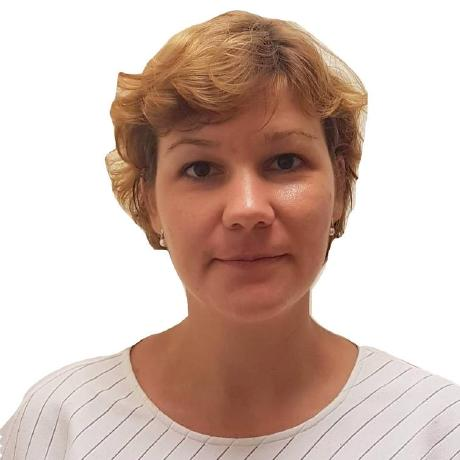
\includegraphics[height=0.35\textheight, width=\linewidth, keepaspectratio]{prof.png}
\end{minipage}

\end{document}